\documentclass[a4paper, 10pt]{report}

% Packages
\usepackage[italian]{babel}
\usepackage[utf8]{inputenc}
\usepackage[T1]{fontenc}
\usepackage{textcomp}
\usepackage{gensymb}
\usepackage{graphicx}
\usepackage{default}
\usepackage{bbding}
\usepackage{hyperref}
\usepackage{amssymb}


% Some heading
%
\includegraphics[height=1.2cm]{images/unipd.png}



%-----------------------------------------------------------------------
% Documento
%-----------------------------------------------------------------------
\begin{document}
% Title page
\title{Analisi di dati relativi ad un\\servizio di bike sharing}
\author{Marco Zanella}
\maketitle

%\tableofcontents



%-----------------------------------------------------------------------
% Abstract
%-----------------------------------------------------------------------
\begin{abstract}
  I sistemi di \emph{bike sharing} sono la nuova generazione di noleggio di
  biciclette completamente automatizzato. Grazie a loro, gli utenti
  sono in grado di noleggiare una bicicletta presso una rastrelliera
  e depositarla successivamente in una qualunque altra. Attualmente in tutto il
  mondo esistono più di 500 programmi di \emph{bike sharing}, i quali
  destano un grande interesse per via del loro impatto su traffico,
  sull'ambiente e sulla salute.
  
  Le attività legate al \emph{bike sharing} sono, inoltre, oggetto di studio
  in ambiti come la ricerca operativa e la statistica, data l'enorme quantità
  di dati che essi generano.
\end{abstract}



%-----------------------------------------------------------------------
% Analisi preliminare
%-----------------------------------------------------------------------
\chapter{Analisi preliminare}
\section{Dataset}
Il dataset utilizzato in questa analisi è stato ottenuto dall'
\href{http://archive.ics.uci.edu/ml}{UCI Machine Learning Repository},
da un lavoro di Hadi Fanaee-T and Joao Gama (\cite{fanaee2013}).

L'utilizzo dei servizi di bikesharing è fortemente influenzato dal
contesto ambientale e climatico. Ad esempio condizioni meteorologiche,
temperatura e orario possono incidere sulla tendenza degli utenti a
noleggiare una bicicletta. I dati sono forniti dal sistema Capital
Bikeshare, Wshington D.C., USA, disponibili al pubblico all'indirizzo
\url{http://capitalbikeshare.com/system-data}, e coprono un'intervallo
di due anni: 2011 e 2012. Gli autori del dataset hanno aggregato i dati
su basi giornaliera ed oraria e, successivamente, hanno inserito informazioni
sulle condizioni meteorologiche (ottenute da \url{http://www.freemeteo.com}).

Lo scopo dell'analisi proposta è predire il numero totale di utenti per
fascia oraria in funzione delle variabili ambientali presenti nel dataset.
Questo risultato consentirà una migliore distribuzione delle biciclette nelle
rastrelliere ed una migliore organizzazione delle operazioni di manutenzione,
facendo in modo che siano effettuate nei periodi di minore utilizzo del servizio.



%-----------------------------------------------------------------------
\section{Significato delle variabili}
Il dataset è suddiviso in due file. Il primo contiene informazioni circa numero
di utenti su base oraria, il secondo contiene le stesse informazioni aggregate
su base giornaliera. La Tab. \ref{tab:variable-meaning} mostra i campi
del dataset e la relativa tipologia. Per le varibili categoriche, viene indicato
tra parentesi il numero di modalità.

\begin{table}
  \centering
  \begin{tabular}{|| c | l | c ||}
    \hline
    Campo       & Descrizione                      & Tipologia       \\ \hline
    \hline
    instant     & ID                              & numerico        \\ \hline
    dteday      & data                            & data            \\ \hline
    season      & stagione                        & categorico (4)  \\ \hline
    yr          & anno                            & categorico (2)  \\ \hline
    mnth        & mese                            & categorico (2)  \\ \hline
    hr          & ora                             & categorico (24) \\ \hline
    holyday     & festività                       & categorico (2)  \\ \hline
    weekeday    & giorno della settimana          & categorico (7)  \\ \hline
    workingday  & giorno lavorativo               & categorico (2)  \\ \hline
    wheaterlist & condizioni meteorologiche       & categorico (4)  \\ \hline
    temp        & temperatura normalizzata        & continuo        \\ \hline
    atemp       & temp. percepita normalizzata    & continuo        \\ \hline
    hum         & umidità normalizzata            & continuo        \\ \hline
    windspeed   & velocità del vento normalizzata & continuo        \\ \hline
    casual      & numero di utenti occasionali    & numerico        \\ \hline
    registered  & numero di utenti registrati     & numerico        \\ \hline
    cnt         & numero di utenti totale         & numerico        \\ \hline
  \end{tabular}
  \caption{Significato delle variabili}
  \label{tab:variable-meaning}
\end{table}

Le variabili \emph{instant} e \emph{dteday} rappresentano un
identificatore numerico assegnato dal sistema di misurazione, non
utile ai fini dell'analisi, e la data nella quale la misura è stata effettuata,
nel formato "yyyy-mm-dd". Anno e mese sono già disponibili come variabili
separate, inoltre è ragionevole assumere che il giorno del mese non
sia utile per predire il numero di utenti, quindi anche questa variabile
può essere trascurata.

La variabile \emph{season} può essere vista come un'aggregazione di
\emph{mnth}: quest'ultima è più precisa, dunque più informativa.
L'intuizione è confermata dalla Fig. \ref{fig:month-season}, che confronta
i boxplot utenti versus mese e stagione, rispettivamente. Nell'ottica di
quest'analisi, è utile mantenere la variabile \emph{season}: l'azienda
che gestisce il servizio ha maggiore interesse ai dati su base trimestrale
che non mensile.

\begin{figure}
  \centering
  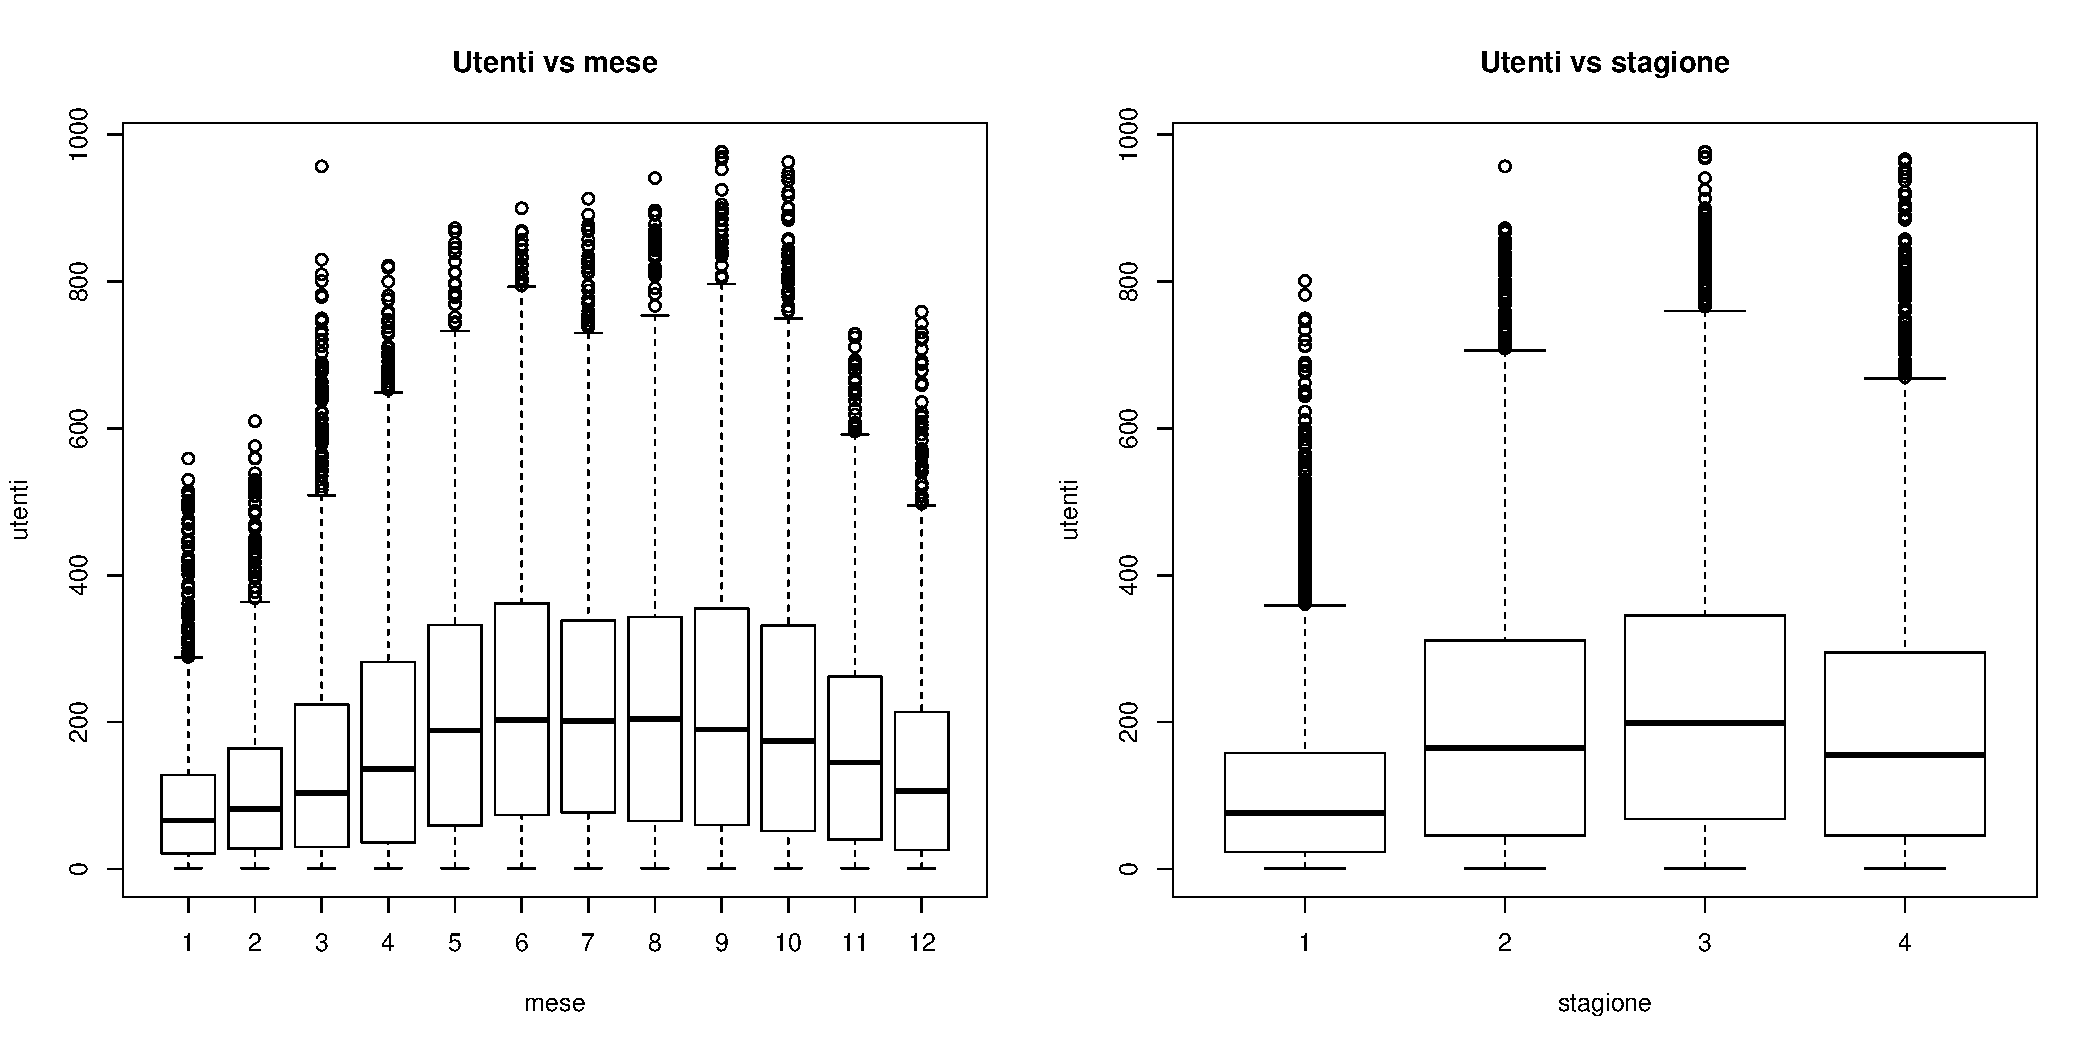
\includegraphics[width=0.95\textwidth]{../plots/month-season.pdf}
  \caption{Utenti in funzione di mesi (sinistra) e stagione (destra)}
  \label{fig:month-season}
\end{figure}

Un ragionamento analogo può essere fatto sull'orario, aggregando le
informazioni per costruire delle fasce. Un criterio di raggruppamento
consiste nel suddividere la giornata tenendo conto del numero di utenti
per fascia, ovvero raggruppando le ore con un numero di utenti simile.
In questa analisi viene proposta una suddivisione in 6 fasce basate
sull'utilizzo del servizio: \emph{molto alto}, \emph{alto}, \emph{medio},
\emph{basso}, \emph{molto basso} e \emph{trascurabile}. Questo tipo di
operazione viene chiamata \emph{clustering}, e non è stata trattata durante il
corso. Tuttavia questo è un caso particolarmente semplice: si vogliono
creare 6 gruppi all'interno di un insieme di 24 elementi, i quali
rappresentano il numero medio di utenti in un determinato orario. Per
quest'operazione si è scelto di utilizzare il metodo \emph{K-means},
del quale è disponibile una descrizione più approfondita nell'Appendice
\ref{app:k-means}. La Fig. \ref{fig:hour-timeslot} mostra il risultato
dell'aggregazione, confrontandolo con il grafico utenti versus orario.

\begin{figure}
  \centering
  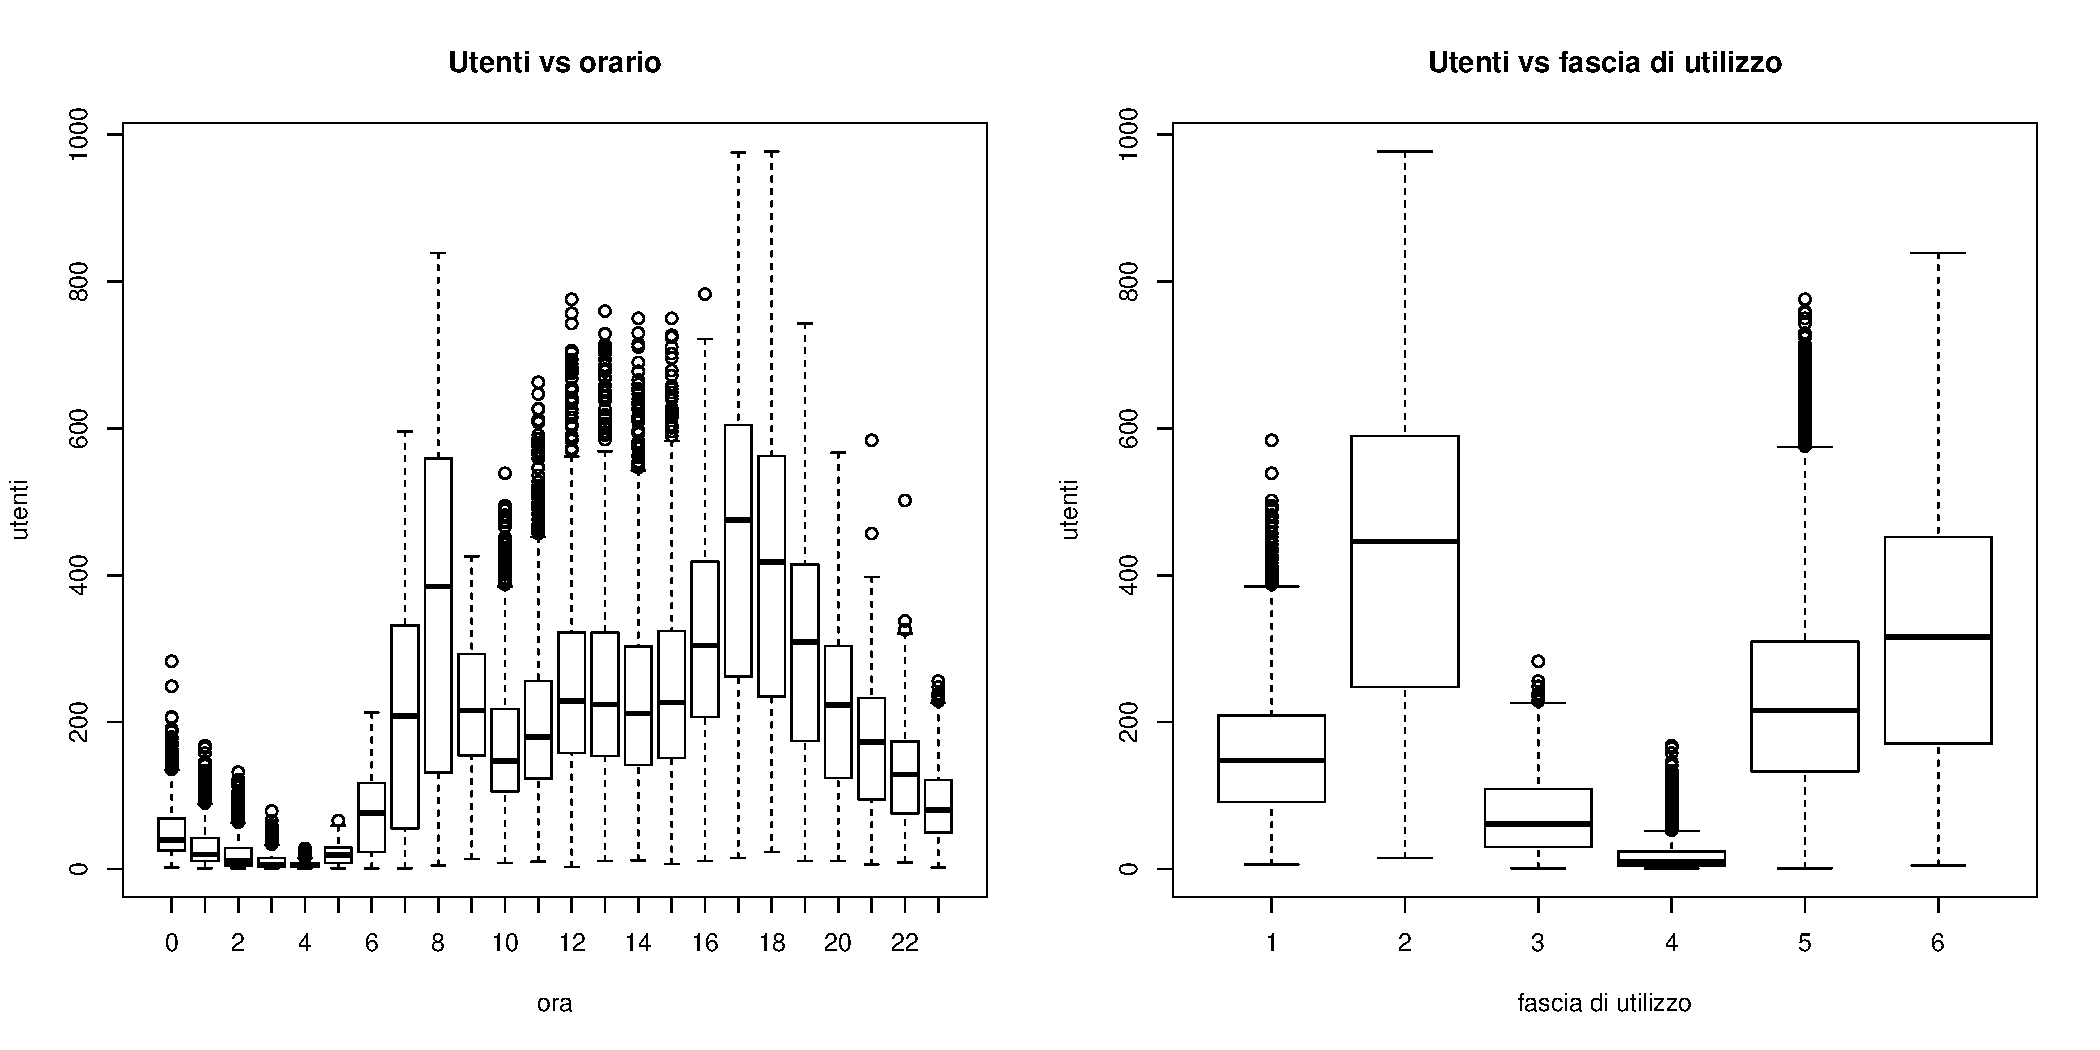
\includegraphics[width=0.95\textwidth]{../plots/hour-timeslot.pdf}
  \caption{Utenti in funzione di orario (sinistra) e fascia di utilizzo (destra)}
  \label{fig:hour-timeslot}
\end{figure}

La Fig. \ref{fig:temperature-humidity} (sinistra) mostra la relazione tra
temperatura percepita e temperatura: sono fondamentalmente identiche,
dunque è sufficiente mantenerne una sola.

\begin{figure}
  \centering
  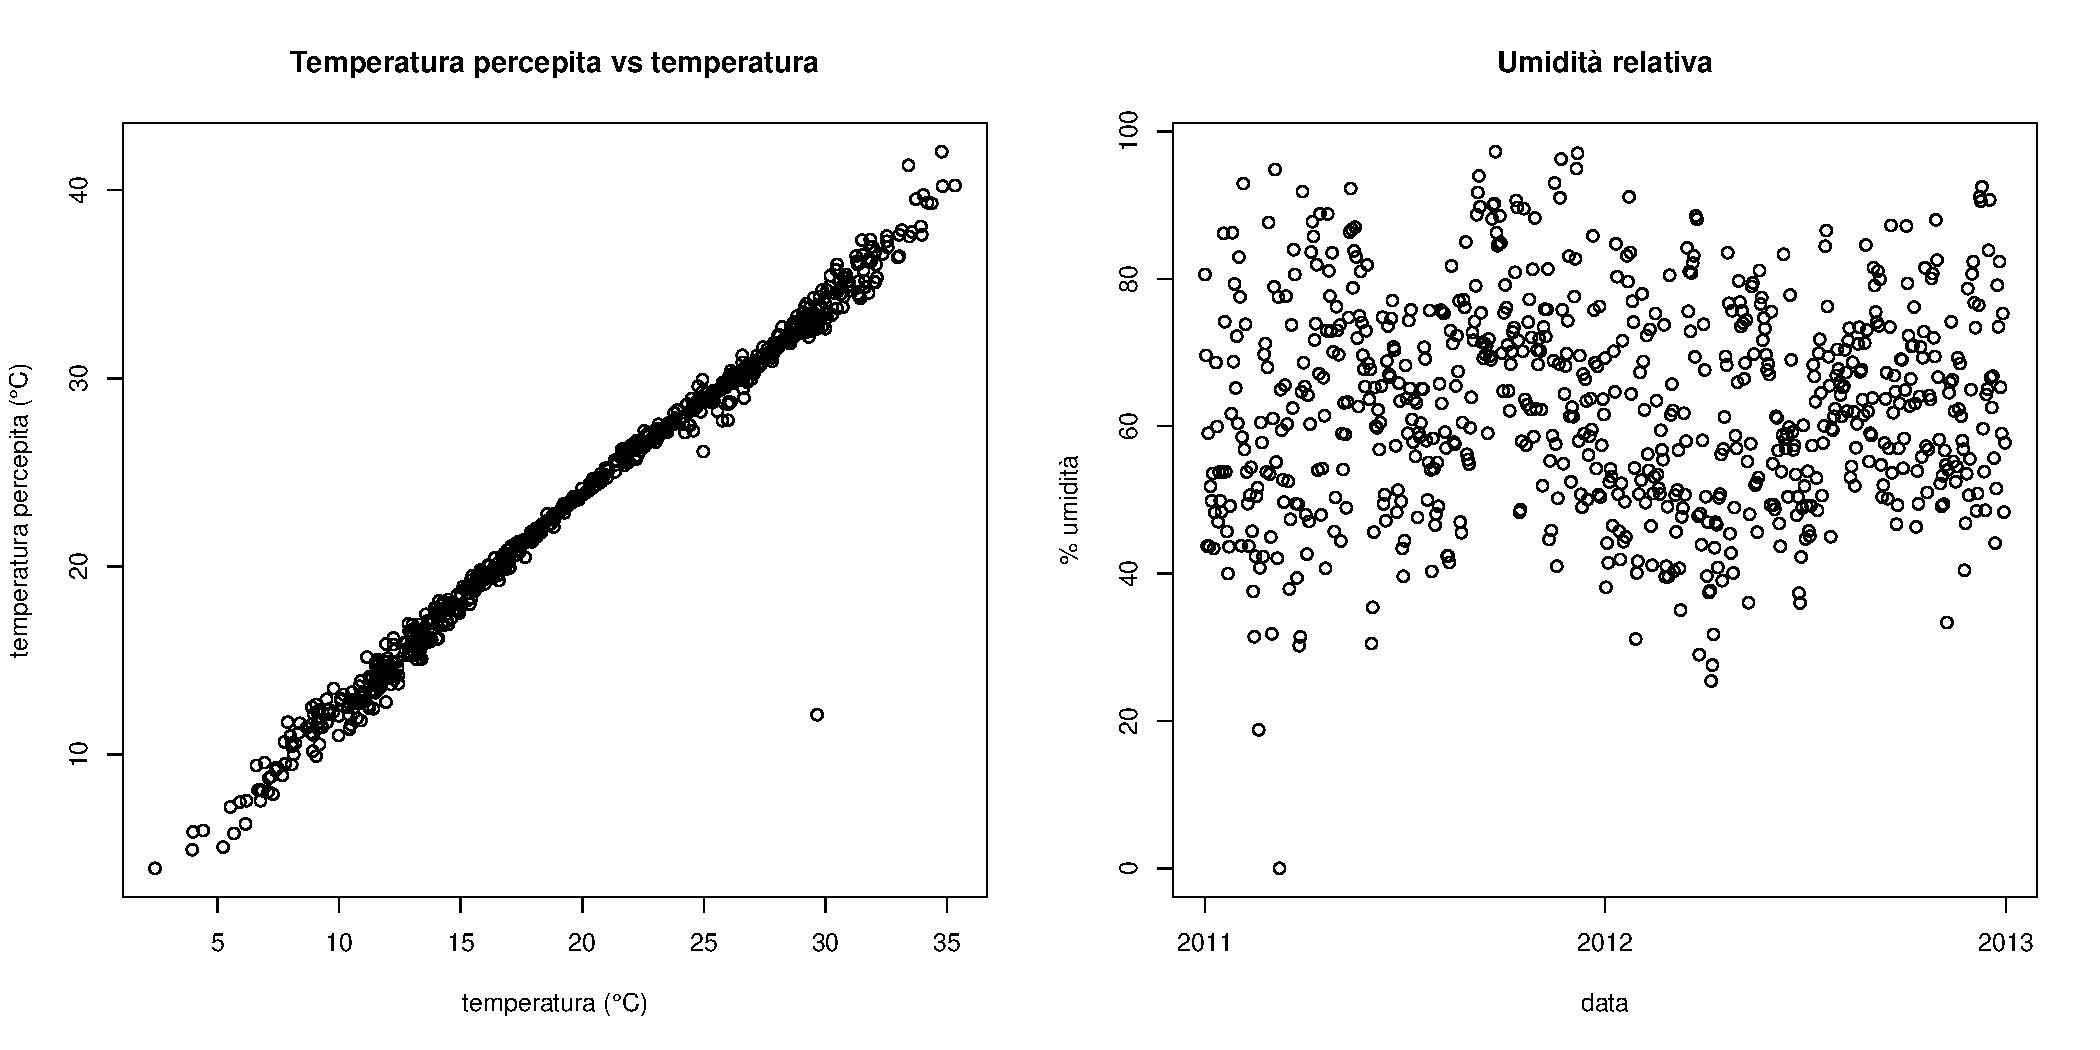
\includegraphics[width=0.95\textwidth]{../plots/temperature-humidity.pdf}
  \caption{Temperatura percepita in funzione della temperatura (sinistra), e umidità (destra)}
  \label{fig:temperature-humidity}
\end{figure}

La variabile \emph{wheaterlist} ha quattro modalità: tempo \emph{sereno},
\emph{incerto}, \emph{pioggia} e \emph{tempesta}. In quest'ultima cadono
solo 3 osservazioni, per cui è opportuno unirla alla terza modalità.



%-----------------------------------------------------------------------
\section{Individuazione degli outlier}
La Fig. \ref{fig:temperature-humidity} (destra) mostra che la percentuale
di umidità varia tra il 10 ed il 100\%, ad eccezione di un punto per cui
la percentuale di umidità è dello 0\%: improbabile dal punto di vista
climatico. Questo punto anomalo rappresenta tutte e sole le misurazioni
del giorno 10 marzo 2011. Molto probabilmente si tratta di un guasto al
sistema, e questo punto è un \emph{outlier}.

Nella Fig. \ref{fig:temperature-humidity} (sinistra) si nota un punto
isolato, per il quale la temperatura percepita è molto bassa: 12.12\degree
contro i 30\degree misurati. Questo punto rappresenta tutte e sole le
osservazioni del giorno 17 agosto 2012. Si tratta probabilmente di un
guasto al rilevatore di temperatura.

Il dataset non contiene informazioni sul 29 ottobre 2012, giorno in cui
l'uragano Sandy ha colpito gli Stati Uniti. Gli autori del dataset hanno
rimosso le misurazioni relative a tale data in quanto non significative.

L'analisi ha rilevato due giornate in cui le misurazioni di temperatura
percepita e umidità sono compromesse. Vista la numerosità del dataset,
è possibile scartare le informazioni di queste due giornate anomale
senza grossa perdita di informazione: 48 osservazioni perse su 17379,
$\approx$ 0.28\%.



%-----------------------------------------------------------------------
% Regressione
%-----------------------------------------------------------------------
\chapter{Regressione}
\label{cap:regression}
Per predire il numero totale di utenti in funzione dei dati disponibili
vengono proposti e confrontati alcuni modelli. L'insieme dei dati è
stato suddiviso in due parti: \emph{insieme di stima} ed \emph{insieme
di verifica}. Il primo serve a costruire ed allenare i modelli, il
secondo a valutarne le prestazioni. L'insieme di stima è ulteriormene
suddiviso in \emph{insieme di costruzione} ed \emph{insieme di controllo}:
il primo per costruire i modelli, il secondo per stimarne eventuali parametri
(ad es. il lisciamento per il loess). Come indice di prestazione viene
utilizzato l'errore quadratico medio (MSE).


%-----------------------------------------------------------------------
\section{Regressione lineare}
Un primo tentativo consiste nel cercare di predire il numero di utenti
in funzione di tutte le altre variabili. Per le variabili esplicative
\emph{isWorkingday} e \emph{timeslot} non sono stati generati coefficienti:
esse sono linearmente dipendenti da \emph{weekday + isHoliday} e \emph{hour},
rispettivamente. Usando l'algoritmo iterativo \emph{stepwise}, si minimizza
l'AIC del modello: nel risultato sono escluse le variabili \emph{isWorkingday}
e \emph{timeslot}. La procedura \emph{stepwise} non riesce ad eliminare
altre variabili, ed il valore $R^{2}$ finale è $\approx$ 0.64, un risultato
soddisfacente considerando la semplicità del modello.

Un secondo approccio consiste nel scegliere manualmente un sottoinsieme
delle variabili da utilizzare. Per questo modello vengono considerate le
variabili \emph{temperature}, \emph{humidity}, \emph{windspeed}, \emph{weather},
\emph{timeslot}, \emph{weekday} e \emph{season}. La scelta è motivata
dalle osservazioni nell'analisi preliminare. Il valore $R^{2}$ è
$\approx$ 0.62, molto vicino a quello del modello precedente.


%-----------------------------------------------------------------------
\section{MARS}
Due modelli MARS sono costruiti sull'insieme di stima. Entrambi selezionano
automaticamente le variabili significative, il secondo opera la scelta
considerando il grado di interazione uguale 2. Quest'ultimo non è stato
trattato esplicitamente durante il corso: come nel MARS con grado di
interazione 1, l'aggiunta di nuove funzioni base avviene scegliendo tra
formule nella forma $c_i \cdot max(0, x - q)$, in più vengono considerate
formule nella forma $c_i \cdot max(0, x_1 - q_1) \cdot max(0, x_2 - q_2)$.


%-----------------------------------------------------------------------
\section{GAM}
Un terzo gruppo di modelli comprende GAM creati sull'insieme di costruzione.
Due criteri di lisciamento sono applicati alle variabili continue:
\emph{splines} e \emph{loess}. Per ciascuna delle due famiglie sono
creati un modello che considera tutte le variabili, ed uno contenente
solo quelle più significative. La significatività è ottenuta dall'analisi
della varianza e dalle osservazioni preliminari.

Il valore del parametro di lisciamento è determinato da una scansione
che minimizza l'MSE sull'insieme di controllo. Il risultato è mostrato
nella Fig. \ref{fig:GAM}.

\begin{figure}
  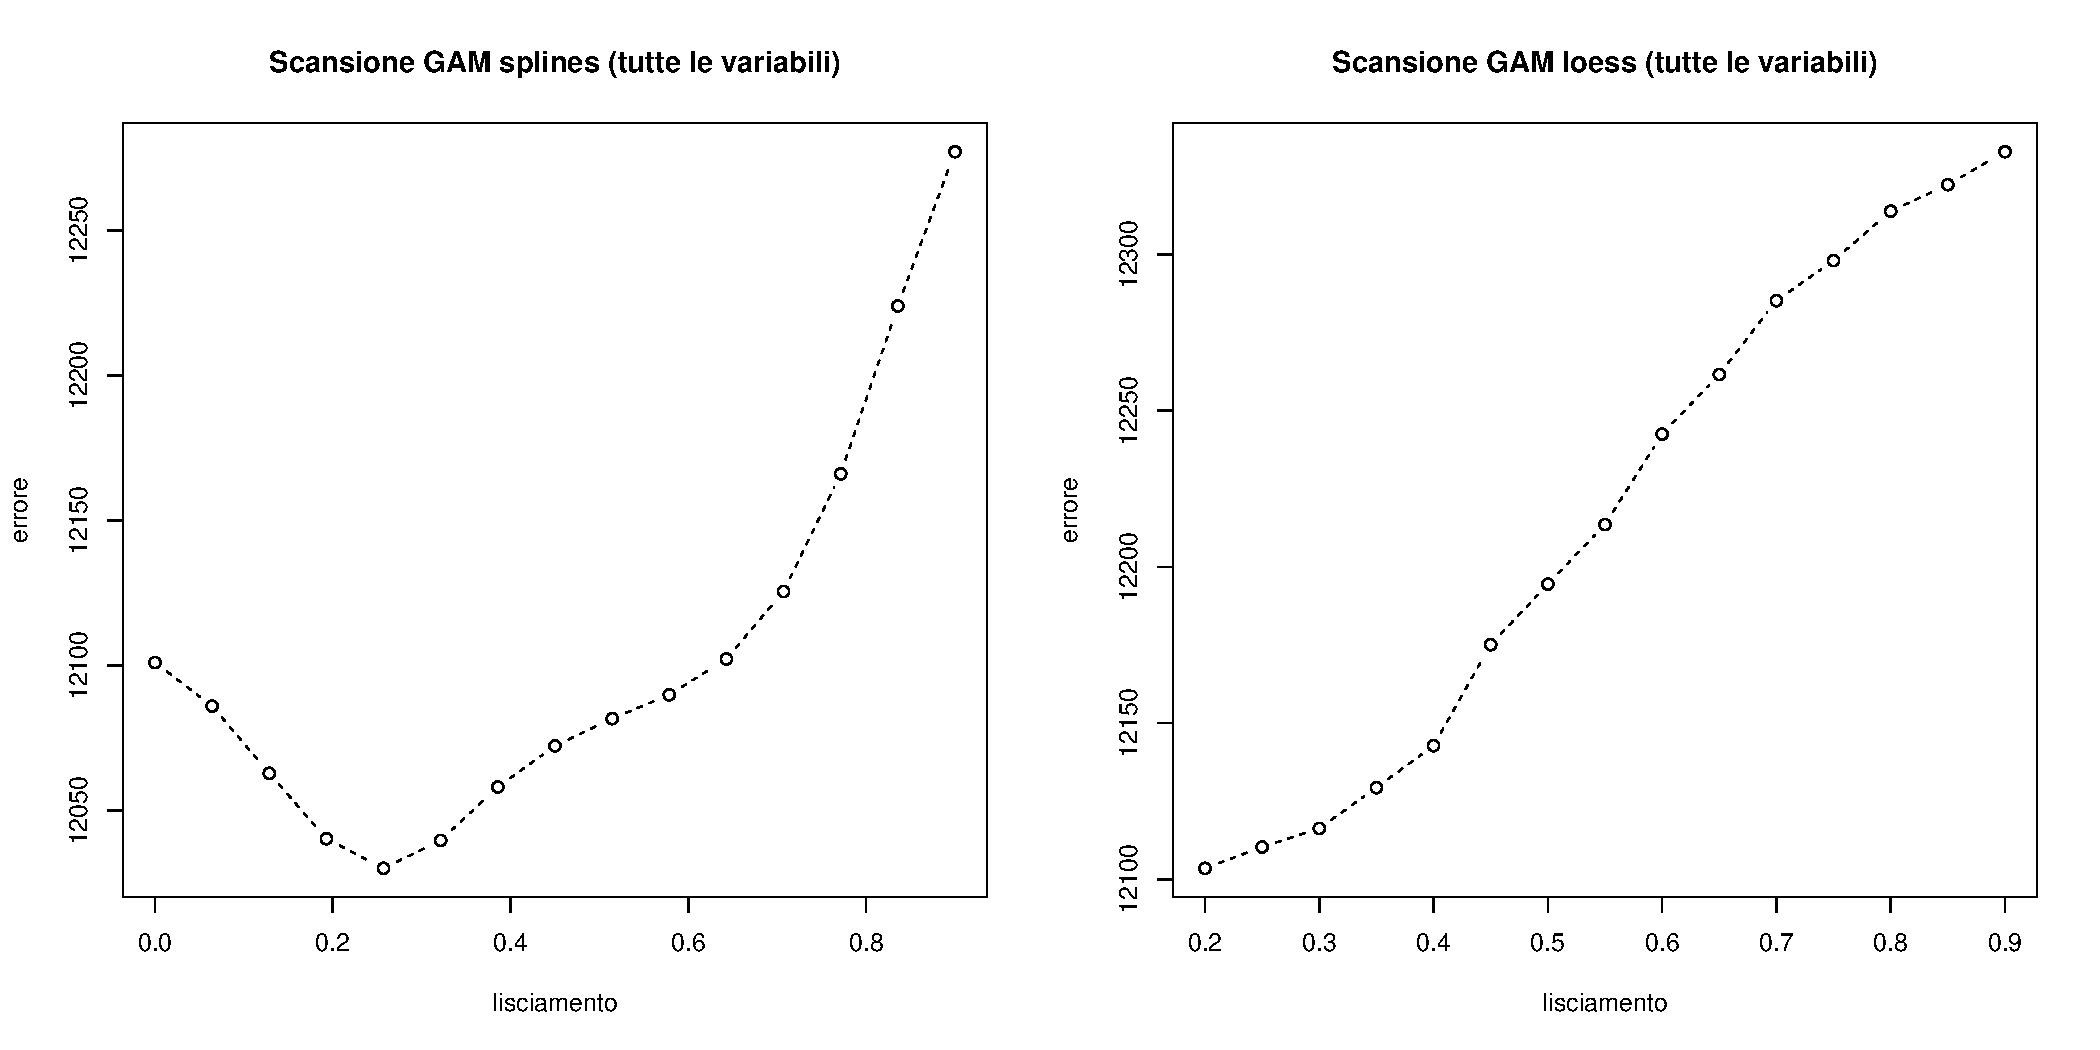
\includegraphics[width=1.0\textwidth]{../plots/GAM.pdf}
  \caption{MSE in funzione del parametro di lisciamento per il GAM con splines (sinistra) e loess (destra)}
  \label{fig:GAM}
\end{figure}

Per non complicare l'analisi, alle variabili continue si impone lo stesso
parametro di lisciamento, anziché stimarne uno diverso per ognuna. La
scelta è motivata dall'elevato costo computazionale della scansione
completa ($\Theta(n^{3})$ contro $\Theta(n)$ di quella proposta).
I risultati ottenuti suggeriscono inoltre che la scansione completa non
apporterebbe un beneficio significativo.


%-----------------------------------------------------------------------
\section{Regressione Projection Pursuit}
Una Regressione Projection Pursuit è applicata ai dati dell'insieme
di costruzione. La PPR si basa su un meccanismo analogo all'analisi delle
componenti principali, seleziona automaticamente le variabili una
volta effettuate le proiezioni e utilizza un parametro per il controllo
del lisciamento.

Il massimo numero di termini ed il parametro di lisciamento sono stimati
minimizzando l'MSE sull'insieme di controllo con una scansione il cui
risultato è mostrato nella Fig. \ref{fig:PPR-NN} (sinistra).

\begin{figure}
  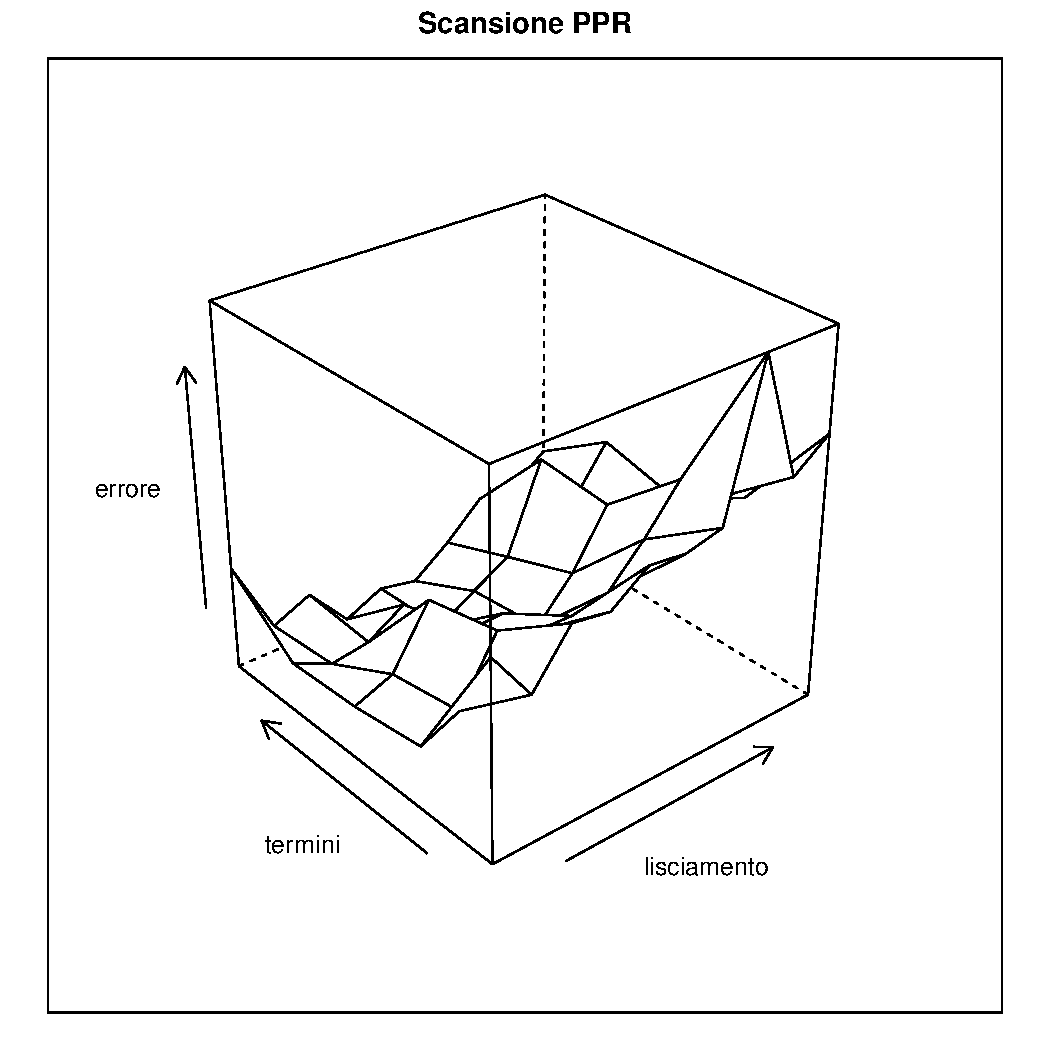
\includegraphics[width=0.45\textwidth]{../plots/PPR.pdf}
  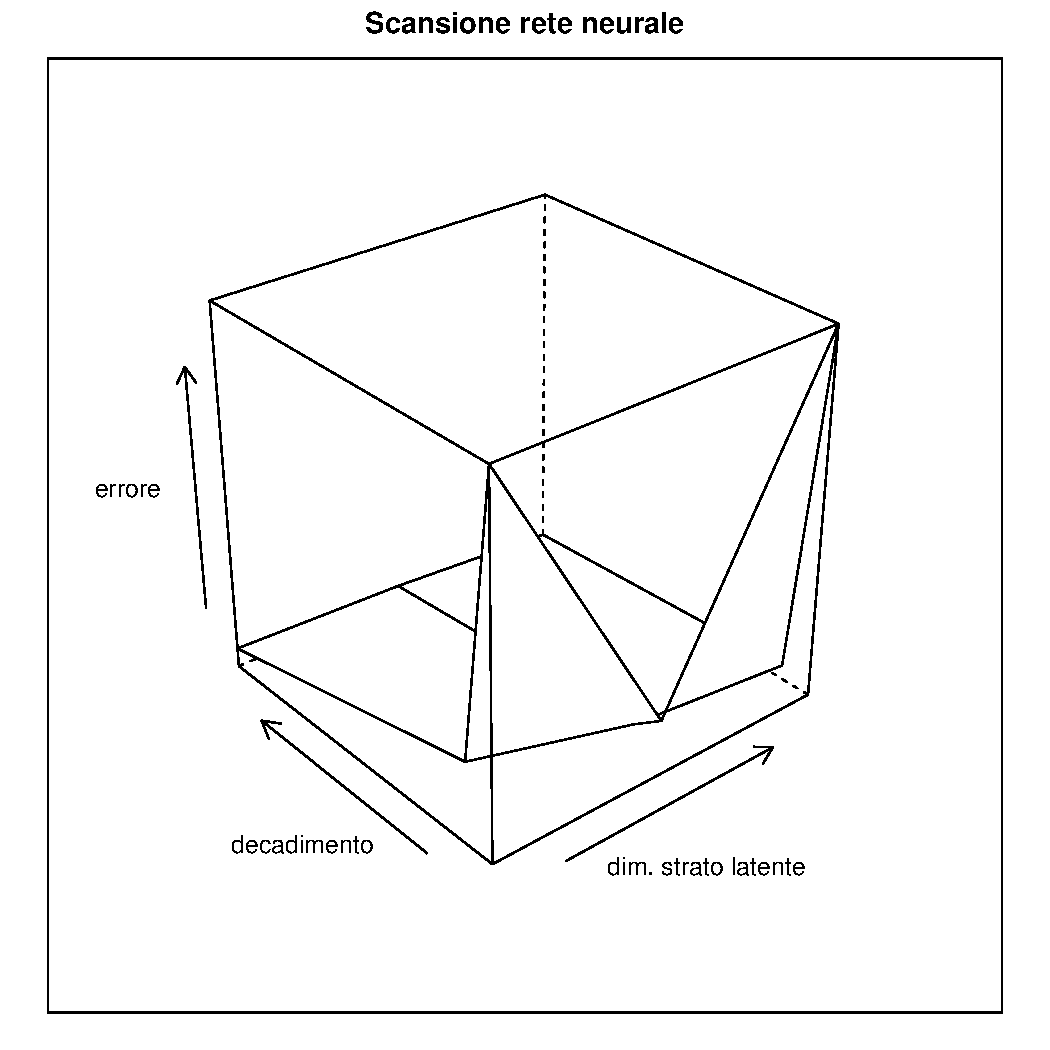
\includegraphics[width=0.45\textwidth]{../plots/neuralnetwork.pdf}
  \caption{
    MSE in funzione di parametro di lisciamento e numero di termini della PPR (sinistra),
    e di dimensione dello strato latente e decadimento per la rete neurale (destra)
  }
  \label{fig:PPR-NN}
\end{figure}


%-----------------------------------------------------------------------
\section{Rete neurale}
Una rete neurale è allenata sull'insieme di costruzione. Una scansione
stima la dimensione dello strato latente ed il valore di decadimento,
minimizzando l'MSE sull'insieme di controllo. La Fig. \ref{fig:PPR-NN}
(destra) mostra il risultato della scansione.

La scansione è fortemente limitata dal tempo di esecuzione dell'allenamento
della rete neurale.



%-----------------------------------------------------------------------
\section{Albero CART}
Un albero CART viene fatto crescere sull'insieme di stima e,
successivamente, potato minimizzandone la devianza (Fig.
\ref{fig:CART} (destra)). L'informazione sulla devianza in funzione del
numero di foglie è ottenuta tramite convalida incrociata. La Fig.
\ref{fig:CART} (sinistra) mostra l'albero dopo la potatura.

\begin{figure}
  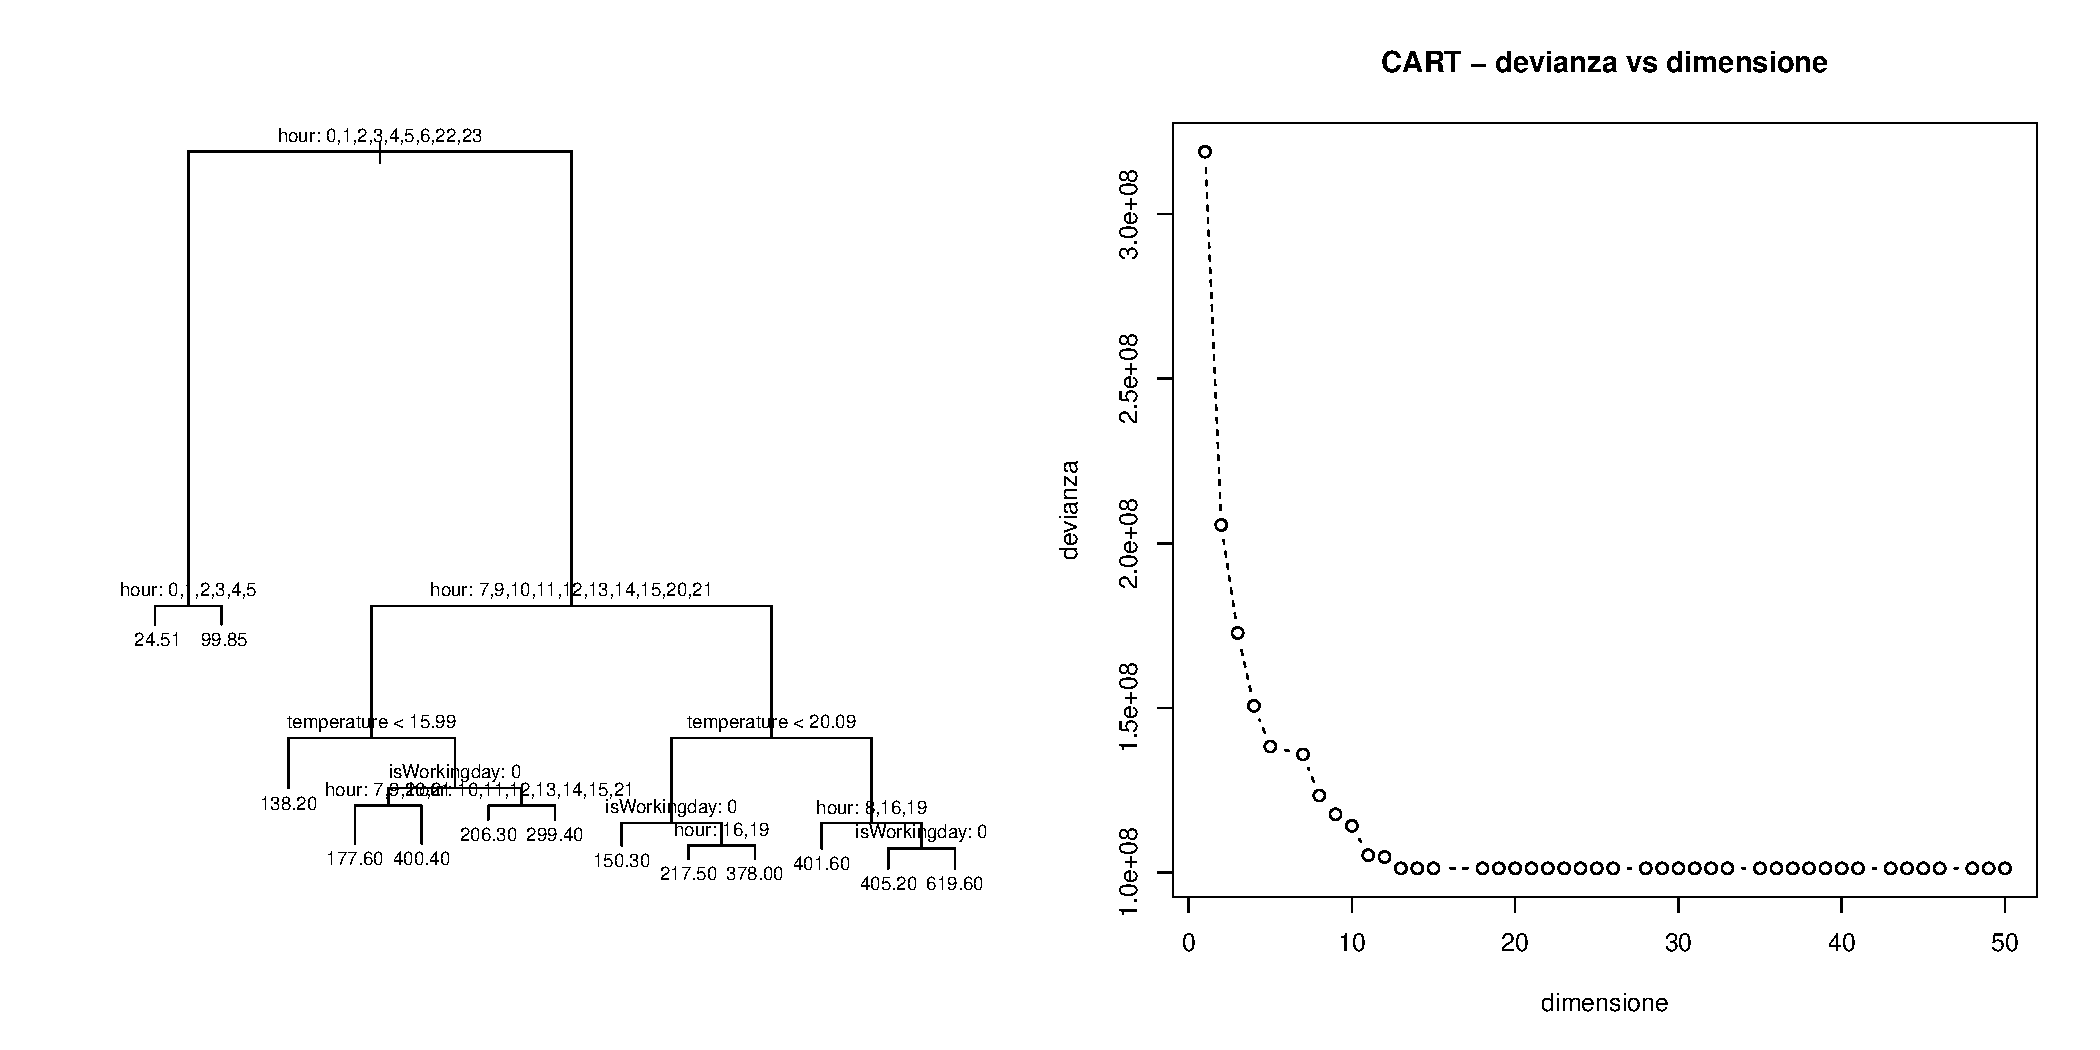
\includegraphics[width=1.0\textwidth]{../plots/CART.pdf}
  \caption{
    CART dopo la potatura (sinistra) e
    devianza vs dimensione (destra)
  }
  \label{fig:CART}
\end{figure}


%-----------------------------------------------------------------------
\section{Confronto e discussione}
La Tab. \ref{tab:comparison} riporta le prestazioni dei modelli proposti,
sotto forma di errore quadratico medio sull'insieme di verifica.

Gli MSE dei modelli sono relativamente simili, sebbene quelli che
considerano le interazioni tra variabili (MARS con grado 2, PPR, rete
neurale e CART) mostrino prestazioni migliori. La PPR in particolare
fornisce l'errore minimo.

La rete neurale ha un errore contenuto, ma ha richiesto un tempo di
calcolo notevole. Il CART fornisce le stesse prestazioni, ma con un
tempo di calcolo più basso. Nel caso in cui si voglia ripetere
l'analisi con nuovi dati, il CART è preferibile alla rete neurale.

I risultati dei modelli lineare e GAM mostrano che la scelta manuale dei
predittori non peggiora significativamente il modello: le analisi
preliminari sono state utili per ridurre la dimensionalità dei dati.

Dal punto di vista della facilità di lettura, i modello migliore è il CART
dopo la potatura: con 13 foglie è in grado di predire bene i dati e di
fornirne un'interpretazione visiva. I modelli lineari e GAM sono
leggermente più difficili da interpretare e hanno un MSE più alto, ma
sono comunque degni di nota.

\begin{table}
  \centering
  \begin{tabular}{|| l | r | r ||}
    \hline
    modello       & variabili       & MSE      \\
    \hline \hline
    Lineare       & tutte           & 12664.50 \\
    Lineare       & solo sign.      & 13056.61 \\
    MARS          & tutte (grado 1) & 12619.53 \\
    MARS          & tutte (grado 2) &  6596.50 \\
    GAM (splines) & tutte           & 12643.32 \\
    GAM (splines) & solo sign.      & 12998.99 \\
    GAM (loess)   & tutte           & 12602.14 \\
    GAM (loess)   & solo sign.      & 12975.89 \\
    PPR           & 6 termini       &  5206.72 \\
    Rete neurale  & -               &  9172.46 \\
    CART          & 50  foglie      &  7347.62 \\
    CART          & 13  foglie      & 10449.94 \\
    \hline
  \end{tabular}
  \caption{Risultati ottenuti dai diversi modelli}
  \label{tab:comparison}
\end{table}





%-----------------------------------------------------------------------
% Appendici
%-----------------------------------------------------------------------
\appendix
%-----------------------------------------------------------------------
\chapter{Caso di studio: classificazione}
\label{app:classification}
Uno scopo secondario dell'analisi è la classificazione degli utenti in
\emph{registrati} e \emph{occasionali}. Dal punto di vista aziendale,
i clienti registrati sono una fonte stabile e costante di guadagni: è
utile identificare i clienti occasionali e "trasformarli" in registrati,
ad esempio stimando in quali momenti la percentuale di utenti occasionali
è più alta (finesettimana, mesi estivi...) per proporre loro abbonamenti
mirati.

Il dataset viene arricchito con un nuovo campo:
$pCasual_i = \frac{casual_i}{total_i}$, il quale rappresenta, per ogni
osservazione, la percentuale di utenti occasionali sul totale. Questo
valore può anche essere letto come la probabilità che un utente coinvolto
in un'osservazione sia un utente occasionale.

Anziché concentrarsi sulla probabilità analitica, le probabilità vengono
classificate come $low$, $medium$ e $high$ sulla base di due soglie. Per
semplicità, le soglie vengono stimate come il primo ed il terzo quartile
della distribuzione di $pCasual$ nel dataset.

Conoscendo i veri valori \emph{pCasual} e \emph{total}, si può predire con
esattezza:
\begin{equation}
  casual_i = pCasual_i \cdot total_i
\end{equation}
Avendo a disposizione uno stimatore per $total$, si può scrivere:
\begin{equation}
  \widehat{casual_i} = pCasual_i \cdot \widehat{total_i}
\end{equation}
Introducendo un'ulteriore approssimazione, si considera la classe di
un'osservazione anziché la probabilità analitica:
\begin{equation}
  \widehat{casual_i} = \widehat{total_i} \cdot \sum\limits_{j \in C} {w_j \cdot c_{ij}}
\end{equation}
dove $C = \{low, medium, high\}$ rappresenta l'insieme delle classi di probabilità,
$c_{ij} \in \{0, 1\}$ vale 1 se e solo se l'osservazione $i$ appartiene alla classe $j$, e
$w_j \in \mathbb{R}$ sono pesi associati a ciascuna classe (stimati, ad esempio, ai
minimi quadrati). Per semplicità di notazione, viene considerata la scrittura informale:
\begin{equation}
  \widehat{casual_i} = class_i \cdot \widehat{total_i}
\end{equation}
come equivalente alla precedente. A questo punto si può allenare un
classificatore per stimare $class$.

Per stimare $class$, viene creato un insieme di stima sul quale sono
allenati i seguenti modelli:
\begin{itemize}
  \item modello lineare, con le due soglie
  \item albero CART di classificazione
  \item albero CART di regressione
  \item MARS
  \item bagging con 50 alberi
  \item boosting con 10 alberi
  \item random forest con 50 alberi
\end{itemize}

La Tab. \ref{tab:classification-error} riporta gli errori totali di
classificazione per ciascun modello sull'insieme di verifica.  I
modelli bagging, boosting e random forest mostrano un errore
tendenzialmente più basso degi altri. I modelli lineare, CART e
MARS sono leggermente peggiori, ma non si discostano molto. I
modelli sono inoltre confrontati attraverso le curve lift (Fig.
\ref{fig:lift}) e ROC (Fig. \ref{fig:roc}), le quali confermano
il primato di random forest e bagging. I modelli basati su
alberi hanno il vantaggio aggiuntivo di essere più semplici da
interpretare.

\begin{table}
  \centering
  \begin{tabular}{|| l | r ||}
    \hline
    Modello                & errore \\
    \hline
    lineare                & 0.34   \\
    CART - classificazione & 0.31   \\
    CART - regressione     & 0.31   \\
    MARS                   & 0.34   \\
    bagging                & 0.29   \\
    boosting               & 0.28   \\
    random forest          & 0.26   \\
    \hline
  \end{tabular}
  \caption{Errore totale dei modelli}
  \label{tab:classification-error}
\end{table}

\begin{figure}
  \centering
  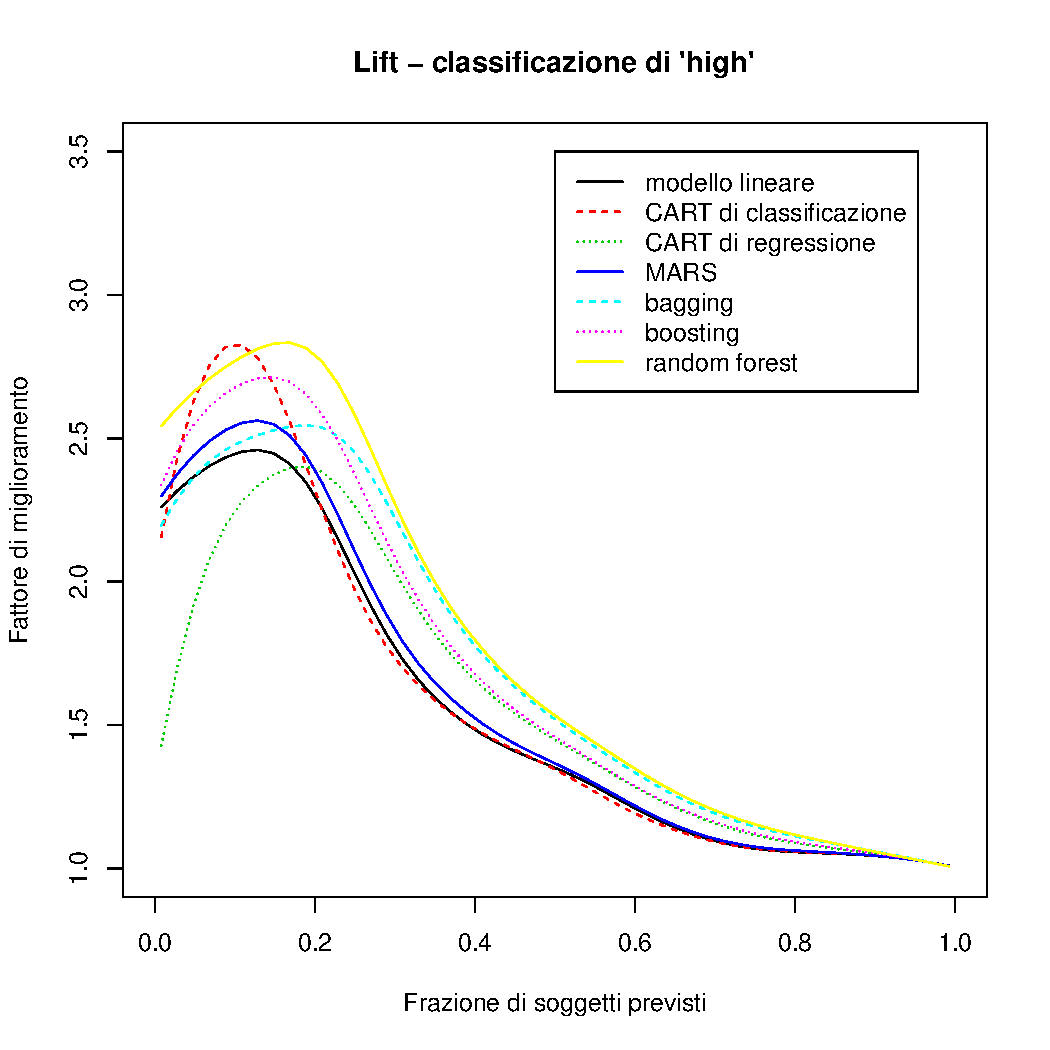
\includegraphics[width=0.49\textwidth]{../plots/lift-high.pdf}
  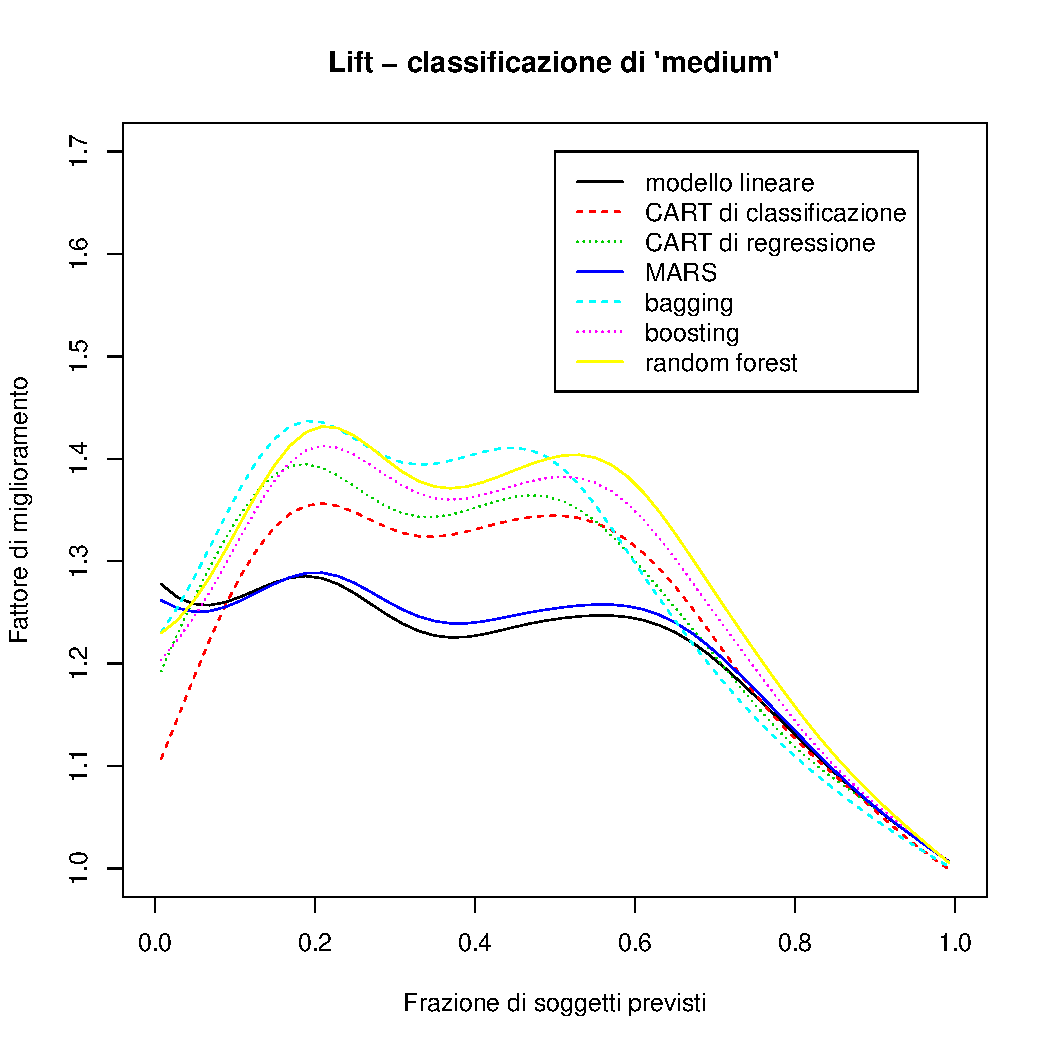
\includegraphics[width=0.49\textwidth]{../plots/lift-medium.pdf}
  \caption{lift per la predizione delle classi \emph{high} (sinistra) e \emph{medium} (destra)}
  \label{fig:lift}
\end{figure}

\begin{figure}
  \centering
  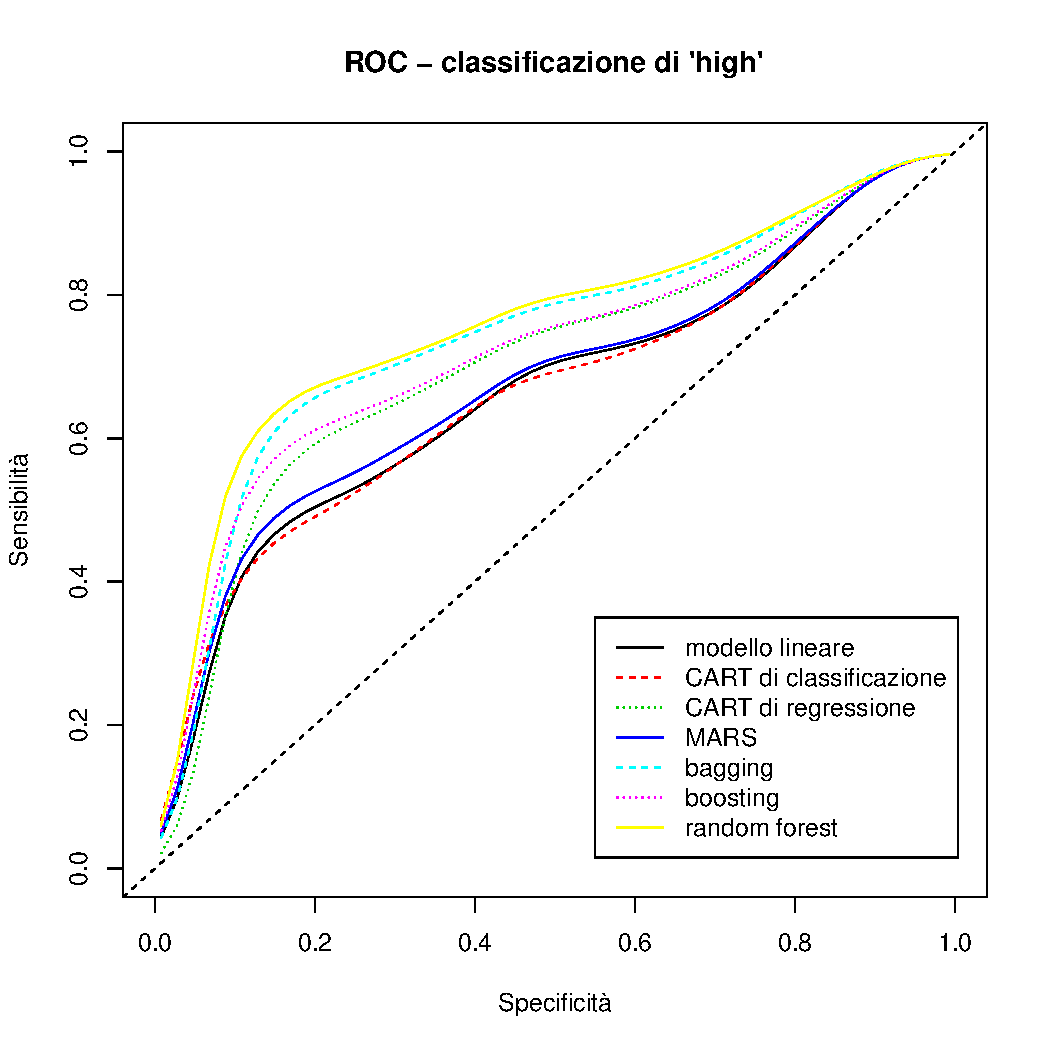
\includegraphics[width=0.49\textwidth]{../plots/roc-high.pdf}
  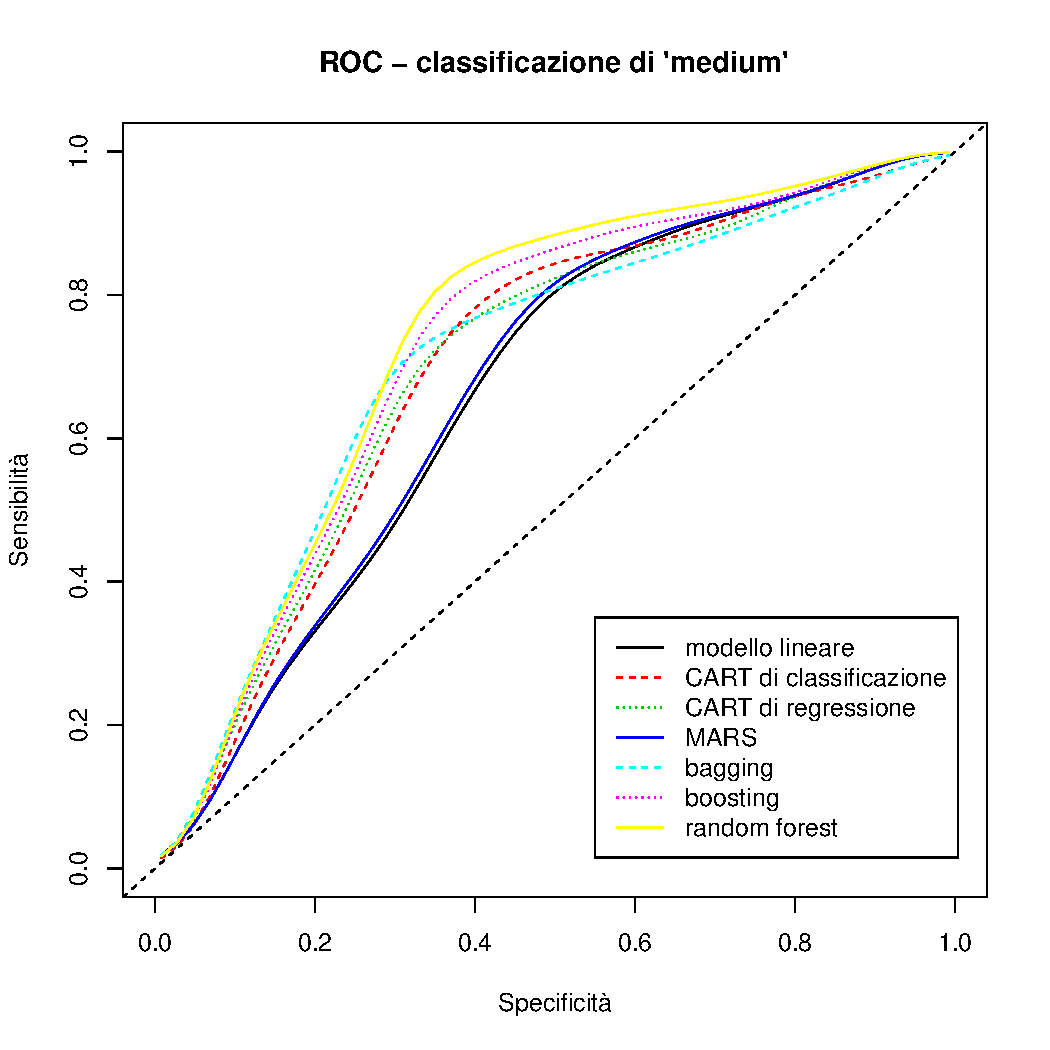
\includegraphics[width=0.49\textwidth]{../plots/roc-medium.pdf}
  \caption{ROC per la predizione delle classi \emph{high} (sinistra) e \emph{medium} (destra)}
  \label{fig:roc}
\end{figure}

Per dare un'idea della qualità della stima proposta, viene costruito un
modello lineare sull'insieme di stima, utilizzando $total$ e $\widehat{class}$
(ottenuto dal bagging) per predire $casual$. Il modello così costruito ha
$R^2 = 89$. L'insieme di verifica (con $\widehat{class}$) viene usato per la
valutazione: la Fig. \ref{fig:classification-residuals} mostra i residui
ottenuti, le linee rosse rappresentano il primo ed il terzo quartile, quelle
blu il decimo e novantesimo percentile: il 50\% degli errori rientra tra
$\pm$15 utenti, l'80\% tra $\pm$27.5 utenti.

\begin{figure}
  \centering
  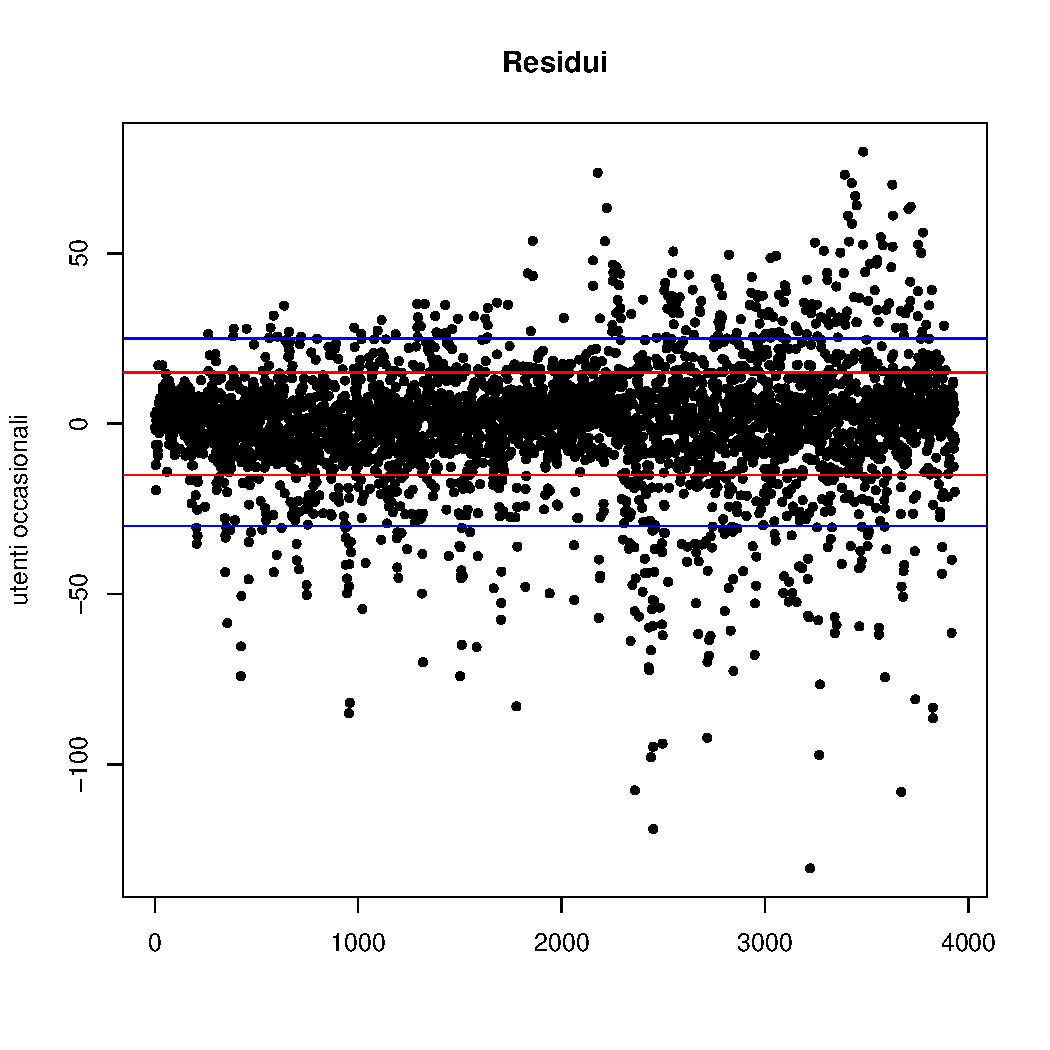
\includegraphics[width=0.5\textwidth]{../plots/classification-residuals.pdf}
  \caption{Residui}
  \label{fig:classification-residuals}
\end{figure}




%-----------------------------------------------------------------------
\chapter{Algoritmo K-means}
\label{app:k-means}
Il \emph{K-means} è un algoritmo di aggregazione non gerarchico,
originariamente pensato per variabili continue. L'idea è raggruppare le
osservazioni \emph{simili}, dove la similarità viene stimata come
distanza euclidea nell'iperspazio delle osservazioni.

L'algoritmo colloca $K$ \emph{centroidi} all'interno dello spazio
delle osservazioni. Ogni osservazione appartiene al gruppo del centroide
più vicino. L'algoritmo procede iterativamente, spostando i centroidi
verso il centro del gruppo che identificano. Gli spostamenti possono
modificare l'appartenenza di un punto ad un gruppo, di conseguenza anche
le posizioni dei centri dei gruppi. La procedura converge ad un punto fisso
quando lo spostamento di un centroide non modifica l'appartenenza dei
punti ad un gruppo.

Nel K-means, il numero di gruppi deve essere noto a priori. È facile
vedere come la scelta di un numero di gruppi inadeguato possa portare
a risultati poco significativi, come in Fig. \ref{fig:kmeans}.

Un altro problema riguarda il criterio di \emph{similarità}: l'algoritmo
la stima come distanza euclidea. Ne consegue che cambiare la scala di
una delle osservazioni modifica il risultato del K-means. Per evitarlo
è necessario riscalare i dati, ma non esiste un modo univoco, in quanto
il concetto di similarità dipende dal particolare problema che si sta
trattando.

Nella sua formulazione di base, inoltre, l'algoritmo non è in grado di
trattare variabili \emph{qualitative}, sebbene esistano delle
generalizzazioni che considerano altre misure di similarità ed il concetto
di \emph{medioide} anziché centroide.

\begin{figure}
  \centering
  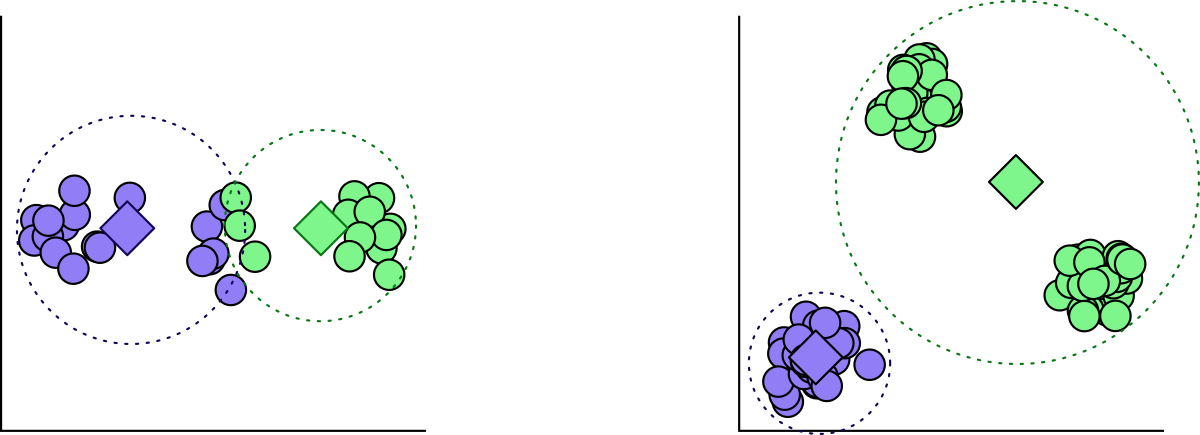
\includegraphics[width=0.95\textwidth]{imgs/kmeans.png}
  \caption{Esempi di K-means con numero di gruppi inadeguato}
  \label{fig:kmeans}
\end{figure}



%-----------------------------------------------------------------------
% Bibliografia
%-----------------------------------------------------------------------
\nocite{azzalini2012data}
\nocite{hastie2013introduction}
\nocite{hastie2005elements}
\bibliographystyle{unsrt}
\bibliography{my_bibliography}

\end{document}